% 	This template is  MIT licensed.

% 	Basic file to demonstrate the usage of this LaTeX template.
% 	You can build your own paper/thesis on top of this file.
% 	Simply adjust the document class and all metadata and start working.
%
\documentclass[
	language=german, % set to english or german
	type=seminar, % set to bachelor, master or seminar
]{isthesis}

% Graphics rendering using TikZ
% See: https://en.wikibooks.org/wiki/LaTeX/PGF/TikZ
\usepackage{tikz}
% Include required TikZ libraries here, some exemplary libraries are pre-included
\usetikzlibrary{calc}
\usetikzlibrary{matrix}
\usetikzlibrary{positioning}
\usetikzlibrary{shapes.geometric}

%Add your library here
\addbibresource{library.bib}

% Import acronyms
% \newacronym[longplural={<long plural>}, shortplural={<short plural>}]{<label>}{<short>}{<long>}
% 	label = is the unique identifier and sort key for the acronym, can be the same as <short>
%	short = is the abbreviation or acronym
%	short plural (optional) = is the plural of the abbreviation or acronym
%	long = is the long form of the acronym, this will appear in the list of abbreviations
%	long plural (optional) = is the long plural form of the abbreviation or acronym

\newacronym[shortplural={KMUen}, longplural={Kleine und Mittlere Unternehmen}]{kmu}{KMU}{Kleines und Mittleres Unternehmen}
\newacronym{CD}{CD}{Corporate Design}
\newacronym{SQL}{SQL}{Structured Query Language}
\newacronym{FAU}{FAU}{Friedrich-Alexander-Universit\"at Erlangen-N\"urnberg}
\newacronym{BPM}{BPM}{Business Process Management}
\newacronym{npm}{NPM}{Node Package Manager}
\newacronym{diss}{DISS}{Digital Industrial Service System}

% Import symbols
% Syntax: <Symbol> <Label> <Name>
% The symbols are sorted by their labels
\addsymboltolist{$\Pi$}{Pi}{Projection}
\addsymboltolist{$\Join$}{Join}{Natural Join}
\addsymboltolist{$\sigma$}{Selection}{Selection}


% Import custom commands
% If you want to define custom commands, please do so here

% Document meta information
\isthesis{
    title={Relaxierung},
    sub-title={Die direkte Methode für nicht-unterhalbstetige Integralfunktionale},
    author-name={Christopher Sorg}, % Separate multiple authors with commas
    author-email={chr.sorg@fau.de},
    principal-supervisor={Prof. Dr. Manuel Friedrich}, % This must be a professor
    group={Lehrstuhl für angewandte Mathematik 1 (Angewandte Analysis)},
    group-institute={Department Mathematik},
    studies={M.Sc. Computational and Applied Mathematics},
    %associate-group={}, % When the thesis is done in cooperation with another chair, add it here
    %associate-group-institute={}, % add cooperating institute or university here
    seminar={Variationelle Probleme für Integralfunktionale}, % The title of your seminar
    submission-date={2022-11-10}, % The date you handed in your document: Format yyyy-mm-dd
    primary-logo={assets/fau-logo.pdf}, % Uses the FAU logo by default
    primary-logo-height={48mm}, % Uses 16mm as default height
    %secondary-logo={}
    secondary-logo-height={0mm} % Uses 16mm as default height
}


\begin{document}
    % Title page
    \newcounter{savepage}
    \maketitle

	% Quote
    % You can put an optional quote page in front of your content
    %   \quotepage[author={Arthur C. Clarke}]{
    %   	        Any sufficiently advanced technology is indistinguishable from magic.
    %   }
    \begin{abstract}
	    % Add your abstract here:
		In diesem Seminar werden verschiedene Aspekte der Variationsrechnung betrachtet. Diese Arbeit setzt die Grundvorlesungen Analysis 1-3, sowie Grundkenntnisse in der Theorie der geometrischen Maßtheorie und \\Funktionalanalysis voraus. Die hieraus benötigten Resultate sind im Zweifel mit passender Quelle im Anhang zu finden.\\
		
		Der erste Bereich beschäftigt sich mit allgemeiner Existenztheorie von Minimierern von Integralfunktionalen. Diese Seminararbeit ist Basis eines 75 minütigen Vortrags, der die Relaxierung behandelt, ein sehr wichtiges Konzept für die angewandte Analysis, da es sich mit der Frage beschäftigt, wie man im Falle von fehlender (schwacher) Unterhalbstetigkeit mit allgemeiner Existenztheorie arbeiten kann.
		
		%Das Buch, das Inspiration und Vorlage für diese Arbeit darstellt, ist unter \cite{Marsden}[§2,Seite 61-86;§5] zu finden. 
	\end{abstract}
    
    % Table of contents
    \tableofcontents

    % List of tables (if you have tables)
    %\listoftables
    
    % List of listings (if you have listings)
	%\lstlistoflistings

    % List of abbreviations (if you use acronyms)
    %\listofabbreviations

    % List of symbols (if you use symbols)
    %\listofsymbols
	
	% Abstract
	%
	% Comment out this part, if you don't require an abstract

	
	% storing the last pagenumber
    \setcounter{savepage}{\value{page}}
    
    
    % Content
    \begin{content}
        % Add your content files:
		\chapter{Einführung}
Die Variationsrechnung ist primär an kritischen Punkten/Minimierern von Funktionalen der Form:
\begin{equation}
    \mathcal{F}: \mathcal{A} \to \overline{\mathbb{R}}
\end{equation}
interessiert. Hierbei bezeichnet \(\mathcal{A}\) einen im Allgemeinen \(\infty-\)dimensionalen Unterraum eines normierten Raumes \(\mathcal{X}\).\\
Bevor wir uns dem eigentlichen Thema zuwenden, werden wir es sowohl mathematisch, als auch physikalisch motivieren. Der mathematischen Motivation dient eine kurze Wiederholung der klassischen direkten Methode. Wiederholung in dem Sinne, dass sie in dem Vortrag zuvor bereits vorgestellt wurde, jedoch von derart großer Bedeutung für das Thema Relaxierung ist, dass wir sie nochmals erwähnen. Im zweiten Teil motivieren wir den Nutzen dann durch ein physikalisches Anwendungsbeispiel.\\

\textbf{Bemerkung:} Insofern nicht explizit angegeben, ist mit Integration immer Integration bezüglich des Lebesgue-/Hausdorff-Maßes gemeint.\\
\section{Wiederholung: Die direkte Methode}
\textit{Quelle für Definitionen/Sätze dieses Kapitels: \cite{CalcVar}}\\[0.1cm]
Zunächst bedienen wir uns einem Lemma, das aus den Analysis-\\Grundlagenvorlesungen schon bekannt sein sollte:\\
\pgfsetfillopacity{0.2}\colorbox{lemyellow}{\begin{minipage}{16cm}{\textcolor{black}{\pgfsetfillopacity{1}}{\label{lem1.1}}}
\textbf{Lemma 1.1 (Cantor's intersection theorem):} Sei \((K_i)_{i \in I}\) eine Familie kompakter Mengen eines Hausdorffraums mit beliebiger Indexmenge \(I\). Dann gilt:
\begin{equation}
    (\bigcap_{i \in J} K_i \neq \emptyset \, \forall J \subset I) \Rightarrow (\bigcap_{i \in I} K_i \neq \emptyset)
\end{equation}
\end{minipage}}

\textsc{Beweis:} Das Lemma ist aus den Grundlagenvorlesungen bekannt und ist auch als duale Version der Überdeckungskompaktheit nicht sehr schwer zu beweisen.\QEDB\\
\\
Nun also die besagte direkte Methode in der allgemeinsten Version:\\
\pgfsetfillopacity{0.2}\colorbox{theored}{\begin{minipage}{16cm}{\textcolor{black}{\pgfsetfillopacity{1}}{\label{theo1.2}}}
\textbf{Satz 1.2 (Die direkte Methode, topologische Version):} Sei \(\mathcal{A}\) ein topologischer, nicht-leerer Hausdorff-Raum, sowie \(\mathcal{F}\) ein Funktional wie in (1.1). Gilt nun:
\begin{enumerate}
    \item Die Subniveaumengen \(\{w \in \mathcal{A}\, | \, \mathcal{F}[w] \le s,\, s \in \mathbb{R}\}\) sind relativ kompakt in \(\mathcal{A}\) und
    \item \(\mathcal{F}\) ist unterhalbstetig auf \(\mathcal{A}\),
\end{enumerate}
dann existiert ein Minimierer \(u \in \mathcal{A}\) von \(\mathcal{F}\).
\end{minipage}}

\textsc{Beweis:} Nach den Voraussetzungen sind die Subniveaumengen kompakt in \(\mathcal{A}\). Diese kann man nun als Schnitt über das Infimum (das \(< \infty\) angenommen werden kann, sonst ist jedes \(u \in \mathcal{A}\) ein Minimierer und die Aussage trivial) betrachten und mit [\ref{lem1.1}][Lemma 1.1] die Behauptung folgern.\QEDB\\

\section{Physikalische Motivation}
\textit{Quelle für Definitionen/Sätze dieses Kapitels: \cite{CalcVarBSchmidt}}\\[0.1cm]
Wir betrachten nun das bekannte Segler-Problem und zeigen dann anhand eines Spezialfalls (den man in Literatur/Internet auch unter Bolza-Problem finden kann), wie bei einem realen physikalischen Problem die direkte Methode fehlschlagen kann.\\
Betrachten wir also einen Segler auf einem Fluss \([a,b] \times [-1,1]\) auf \(\{(x,w(x))\, | \, x \in [a,b]\}\) mit Gegenwind \((-1,0)\). Nun wird der Segler am effektivsten segeln, indem er die Windkraft im optimalen Winkel \(\alpha > 0\) ausnutzt. Der Kurs muss also \(|w'(x)|=\alpha\) erfüllen. Wir sind hierbei also an folgendem variationellem Problem interessiert:
\begin{equation}
    \text{max} \leftarrow \mathcal{F}[w]:=\int_{a}^b F(w'(x)) \,dx 
\end{equation}
Diese Modellierung ist sehr idealistisch, da wir nicht die Strömung \(S(w(x))\) des Flusses berücksichtigen. Die bessere Modellierung lautet also:
\begin{equation}
    \text{max} \leftarrow \mathcal{F}[w]:=\int_{a}^b F(w'(x)) + S(w(x))\, dx
\end{equation}
Bildlich könnte man sich diese Situation folgendermaßen vorstellen:
\begin{figure}[!h]
    \centering
    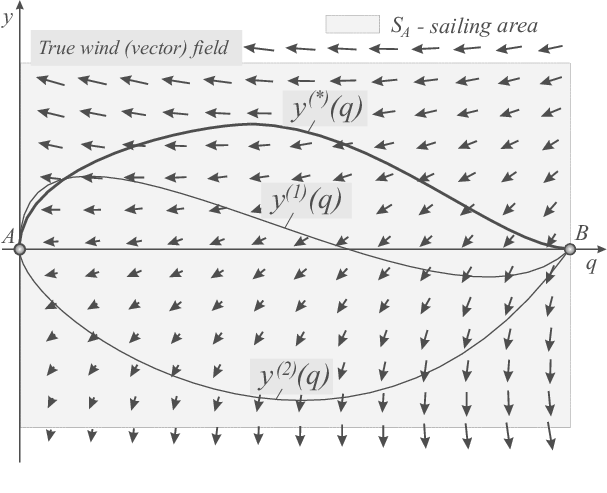
\includegraphics[scale=0.42]{figures/Sailboat-trajectory.png}
    \caption{Graphische Veranschaulichung des Seglerproblems\cite{Sailboat}}
    \label{fig:sail}
\end{figure}\\

Zu sehen sind Beispiele an zulässigen Trajektoren von Punkt A nach Punkt B mit \(y^*(q)\) der approximierten Optimalroute.\\
Wir haben dieses Problem gerade so modelliert, dass die Maxima von F und S \\gerade \(F_{\text{max}} = F(\pm \alpha)\) und \(S_{\text{max}} = S(0)\) sind. Wir sehen also ein, dass das Supremum gegeben ist durch \((F_{\text{max}} + S_{\text{max}})(b-a)\). Dies führt jedoch zu einem Problem, denn damit besitzt das Funktional \(\mathcal{F}\) keinen Maxmierer, da \(u = 0\) f.ü. gelten müsste, weshalb dann \(u' = 0 \neq \pm \alpha\) f.ü. wäre.\\
Doch woran ist die Existenztheorie hier genau gescheitert? Dazu wollen wir nun, wie bereits oben schon einmal erwähnt, den Bolza-Spezialfall (als duale Version des obigen Maximierungsproblems) mathematisch genauer unter die Lupe nehmen:\\
Sei \(a < b \in \mathbb{R}\) und
\begin{equation}
    \mathcal{F}:W^{1,4}(]a,b[) \to \mathbb{R}_0^+,\,\mathcal{F}[w] := \int_{a}^b ((w')^2 - 1)^2 + w^4\,dx
\end{equation}
Da \(W^{1,4}(]a,b[)\) ein Hilbertraum ist, ist er insbesondere ein reflexiver Banachraum. Damit gilt Bedingung (1) der direkten Methode, da \(\mathcal{F}\) Norm-koerziv ist (mit der Young-\\Ungleichung gilt \((w')^2 \le  \frac{(w')^4}{4} + 1\) und in reflexiven Banachräumen (auf einem schwach abgeschlossenem Unterraum; schwach im Sinne der schwachen Topologie (Initialtopologie zum Dual-Raum)) folgt Bedingung (1) der direkten Methode aus Norm-\\Koerzivität; für einen Beweis verweisen wir aus Zeitgründen auf \cite{CalcVar}[Seite 30-31]). \\Allerdings ist das Funktional \textbf{nicht} unterhalbstetig auf \(W^{1,4}_0(]a,b[)\) (und damit insbesondere auch nicht auf \(W^{1,4}(]a,b[)\)) \cite{CalcVarJost}[Seite 206]:\\
Definiere die "Sägezahn-Funktionenfolge"
\begin{equation}
    w_k(x) : = \frac{b-a}{2k} - |x - (a + \frac{a + b}{2k})| \,\, \forall x \in [a,a + \frac{b-a}{k}]
\end{equation}
und setze diese periodisch fort. Es folgt
\begin{equation}
    \mathcal{F}[w_k] \le ||w_k||^4_{\infty} \stackrel{k \to \infty}{\to} 0,
\end{equation}
da unter den Voraussetzungen \(W^{1,\infty}_0(]a,b[) \subset W^{1,p}_0(]a,b[)\) für alle \(p \in [1,\infty]\) gilt. Weiter gilt allerdings
\begin{equation}
    \mathcal{F}[w_k] = k \int_a^{a + \frac{b-a}{k}} w_k^4\, dx \le k \int_a^{a + \frac{b-a}{k}} (\frac{b-a}{2k})^4 \, dx < \mathcal{F}[0] = b - a,
\end{equation}
weshalb \(\mathcal{F}\) nicht Folgen-unterhalbstetig ist. Damit schlägt die Bedingung (2) der direkten Methode fehl und das Funktional hat keinen Minimierer (wie man auch leicht nachrechnet, ist das Infimum auf \(W^{1,4}_0(]a,b[)\) von dem Funktional 0 und dieses kann nicht angenommen werden).
		\chapter{Nicht-Unterhalbstetigkeit und Relaxierung}
\textit{Quelle für Definitionen/Sätze dieses Kapitels: \cite{CalcVarJost}[Seite 208 ff.]}\\[0.1cm]
Wir haben in Kapitel 1 gesehen, dass nicht-unterhalbstetige (uhs) Funktionale nicht abstrakt-künstlicher Natur sind, sondern durchaus in der Anwendung immer wieder auftreten. Wir werden uns deshalb ansehen, wie wir mit solchen Fällen umgehen können. Wir werden in Kapitel 3 dann auch auf das Bolza-Beispiel zurückkommen.\\

\pgfsetfillopacity{0.2}\colorbox{defblue}{\begin{minipage}{16cm}{\textcolor{black}{\pgfsetfillopacity{1}}{\label{def2.1}}}
\textbf{Definition 2.1 (Relaxierung):} Betrachte einen topologischen Raum \((X,\tau)\), kurz \(X\) und ein Funktional \(\mathcal{F}:X \to \overline{\mathbb{R}}\). Dann definieren wir die uhs Einhüllende bzw. das relaxierte Funktional (oder einfach nur Relaxierte) \(sc^- \mathcal{F}\) von \(\mathcal{F}\) durch:
\begin{equation}
    (sc^-\mathcal{F})[x] := \sup \{\Phi[x] \, | \, \Phi : X \to \overline{\mathbb{R}} \text{ ist uhs mit }\Phi[y] \le \mathcal{F}[y] \, \forall y \in X\}
\end{equation}
\end{minipage}}

\textbf{Bemerkung:} Die Relaxierte ist die größte uhs Funktion auf \(X\), die \(\le \mathcal{F}\) ist. Dies entnimmt man direkt der Definition und der Tatsache, dass die Relaxierte uhs als Supremum von uhs Funktionalen ist.\\
Warum man genau die uhs Einhüllende wählt, wird dann im Folgevortrag über \(\Gamma-\\\)Konvergenz noch klar.\\

\begin{figure}[!h]
    \centering
    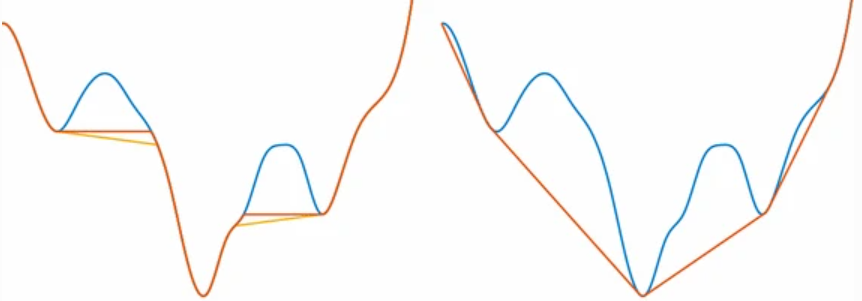
\includegraphics[scale=0.8]{figures/Einhuellende.png}
    \caption{Das Konzept der Einhüllenden: In blau eine gegebene Funktion; quasikonvexe Einhüllende (rot/orange), robust quasikonvexe Einhüllende (gelb) links; konvexe Einhüllende (rot/orange) rechts \cite{ConvexEnvelope}}
    \label{fig:einh}
\end{figure}

Kommen wir nun zurück auf die Ursprungsfrage, wie man im Falle von nicht-\\unterhalbstetigen Funktionalen die Minimierung "reparieren" kann. Der folgende Satz beantwortet diese Frage:\\
\pgfsetfillopacity{0.2}\colorbox{theored}{\begin{minipage}{16cm}{\textcolor{black}{\pgfsetfillopacity{1}}{\label{theo2.2}}}
\textbf{Satz 2.2 (Minimierung durch Relaxierung):} Betrachte einen topologischen Raum \(X\) und ein Funktional \(\mathcal{F}: X \to \overline{\mathbb{R}}\). Es gilt:
\begin{enumerate}
    \item Jeder Häufungspunkt einer Minimierungsfolge von \(\mathcal{F}\) ist ein Minimierungspunkt der Relaxierten.
    \item Ist \(\mathcal{F}\) zusätzlich (Norm-)koerziv, so gilt
        \begin{equation}
            \min_X sc^- \mathcal{F} = \inf_X \mathcal{F}.
        \end{equation}
\end{enumerate}
\end{minipage}}

\textsc{Beweis:} 
\begin{enumerate}
    \item Betrachte also eine Minimierungsfolge \((x_n)_{n \in \mathbb{N}} \subset X\) für \(\mathcal{F}\), i.e. \(\lim_{n \to \infty} \mathcal{F}[x_n] = \inf_X \mathcal{F} < \infty\) (wobei Letzteres wieder o.B.d.A., siehe [\ref{theo1.2}][Satz 1.2]; die Existenz ist eine Konsequenz aus der Definition des Infimums), mit Häufungspunkt \(x_0\). Dann gilt
    \begin{equation}
        (sc^- \mathcal{F})[x_0] \le \liminf_{n \to \infty} (sc^- \mathcal{F})[x_n] \le \liminf_{n \to \infty} \mathcal{F}[x_n] = \inf_{y \in X} \mathcal{F}[y].
    \end{equation}
    Das Infimum aus (2.3) ist eine konstante Abbildung und damit uhs (sogar stetig: Jede beliebige offene Teilmenge der Bildmenge einer konstanten Funktion hat entweder ein leeres Urbild oder die gesamte Definitionsmenge als Urbild; in beiden Fällen impliziert die Definition einer Topologie sofort die Stetigkeit) und nach Definition des Infimums auch \(\le \mathcal{F}\), also gilt nun nach obiger Bemerkung: 
    \begin{equation}
        \inf_{y \in X} \mathcal{F}[y] \le (sc^- \mathcal{F})[x].
    \end{equation}
    Da \(x_0\) beliebig war, ist die erste Behauptung damit gezeigt.
    \item Ist \(\mathcal{F}\) zusätzlich koerziv, so gilt:
    \begin{equation}
        \text{Jede Subniveaumenge }\{w \in \mathcal{A} \subset X\, | \, \mathcal{F}[w] \le s \in \mathbb{R}\} \text{ ist beschränkt},
    \end{equation}
    bzw., falls \(X\) zusätzlich normiert ist, ist das äquivalent zu
    \begin{equation}
        \forall x_n \subset X\text{ mit } \sup_{n} \mathcal{F}[x_n] < \infty:\, \sup_n ||x_n||_{X} < \infty.
    \end{equation}
    Damit ist klar, dass jede (wie obige) Minimierungsfolge einen Häufungspunkt hat, weshalb die 2. Behauptung ebenfalls bewiesen ist.\QEDB\\
\end{enumerate}

\textbf{Bemerkung 1:} Streng genommen haben wir nun nur für die Folgenversion eine Antwort gegeben und deshalb nur im Falle, dass für alle \(x \in X\) eine abzählbare Umgebungsbasis existiert, auch auf die topologische Version. Jedoch ist in der Anwendung normalerweise die Folgenversion die gebräuchliche Version.\\

\textbf{Bemerkung 2:} Die benutzten äquivalenten Formulierungen (2.5) und (2.6) können elementar bewiesen werden. (2.6) ist als Folgenversion klar, (2.5) ist die notwendige Bedingung ebenfalls klar. Für die hinreichende Bedingung wähle Umgebung für die Subniveaumenge klein genug, was dank der Beschränktheit möglich ist.\\

Haben wir tatsächlich einen topologischen Raum vorliegen, der das 1. Abzählbarkeitsaxiom (AA) - siehe obige Bemerkung 1 - erfüllt, können wir uns das Leben für direkte Berechnungen mithilfe von Folgenkriterien deutlich einfacher machen:\\
\pgfsetfillopacity{0.2}\colorbox{lemyellow}{\begin{minipage}{16cm}{\textcolor{black}{\pgfsetfillopacity{1}}{\label{prop2.3}}}
\textbf{Proposition 2.3 (Folgenkriterium für die Relaxierte):} Sei also \(X\) ein topologischer Raum, der das 1.AA erfüllt. Dann ist \((sc^-\mathcal{F})\) das relaxierte Funktional zu \(\mathcal{F}:X \to \overline{\mathbb{R}}\), genau dann wenn gilt:
\begin{enumerate}
    \item \begin{equation}
        (sc^- \mathcal{F})[x] \le \liminf_{n \to \infty} \mathcal{F}[x_n], \, \text{falls }x_n \stackrel{n \to \infty}{\to} x
    \end{equation}
    \item \begin{equation}
        \forall x \in X \,\exists x_n:\, x_n \stackrel{n \to \infty}{\to} x\, \land \, (sc^- \mathcal{F})[x] \geq \lim_{n \to \infty} \mathcal{F}[x_n]
    \end{equation}
\end{enumerate}
\end{minipage}}

\textsc{Beweis:} Es genügt zu zeigen, dass
\begin{equation}
    \inf\{\liminf_{n \to \infty} \mathcal{F}[x_n] \, | \, x_n \stackrel{n \to \infty}{\to} x \text{ in } X\}
\end{equation}
Folgen-unterhalbstetig (als alternative Definition der Relaxierten im Folgensinne) ist, da \(X\) das 1.AA erfüllt und wir für Bedingung (2) dann einfach die passende Minimierungsfolge wählen können.\\
Für (2.9) gilt:
\begin{equation}
    \liminf_{m \to \infty}(\inf\{\liminf \mathcal{F}[y_{m,n}]\, | \, y_{m,n} \to y_m\}) \geq \inf\{\liminf \mathcal{F}[x_n]\, | \, x_n \stackrel{n \to \infty}{\to} x\},
\end{equation}
falls \(y_m \stackrel{m \to \infty}{\to} x\).\\
Angenommen nämlich, (2.10) stimmt nicht, dann gäbe es für ein \(\epsilon > 0\) eine Diagonalfolge \(y_{m,n_m} \stackrel{m \to \infty}{\to} x\) der Doppelfolge \(y_{m,n}\) mit
\begin{equation}
    \mathcal{F}[y_{m,n_m}] < \inf \{\liminf \mathcal{F}[x_n]\, | \, x_n \stackrel{n \to \infty}{\to} x\} - \epsilon
\end{equation}
im Widerspruch zur Definition des Infimums.\\
Nun verbleibt, die Gleichheit von (2.9) und der Relaxierten zu zeigen. Dies folgt aber direkt aus der Definition der Relaxierten, genauer der Bemerkung unterhalb von [\ref{def2.1}][Definition 2.1].\QEDB

Nun wollen wir 2 einfache, aber wichtige Beispiele vorstellen:\\
\pgfsetfillopacity{0.2}\colorbox{propgreen}{\begin{minipage}{16cm}{\textcolor{black}{\pgfsetfillopacity{1}}{\label{ex2.4}}}
\textbf{Beispiel 2.4:} Sei X ein topologischer Raum mit 1.AA, \(B \stackrel{offen}{\subset} X\). Dann gilt:
\begin{enumerate}
    \item \begin{equation}
        \mathbf{1}_B(x) :=\begin{cases} 0, \, x \in B\\ \infty, \, x \notin B\end{cases} \Rightarrow\,sc^- \mathbf{1}_B = \mathbf{1}_{\overline{B}}
    \end{equation}
    \item \begin{equation}
        \chi_B(x) :=\begin{cases} 1, \, x \in B\\ 0, \, x \notin B \end{cases}\Rightarrow\,sc^- \chi_B = \chi_{B^c}
    \end{equation}
\end{enumerate}
\end{minipage}}

\textsc{Beweis:}
Wir werden den Beweis für die Indikatorfunktion durchführen. Der Beweis für die charakteristische Funktion ist komplett analog. Dazu weisen wir die zwei Kriterien aus [\ref{prop2.3}][Proposition 2.3] nach:
\begin{enumerate}
    \item Wir führen eine einfache Fallunterscheidung durch:
    \begin{itemize}
        \item Sei \(x \in B\). Dann gilt:
        \begin{equation}
            \exists n \in \mathbb{N} \, \forall \tilde{n} \geq n \,: \, x_{\tilde{n}} \in \overline{B}.
        \end{equation}
        Also folgt:
        \begin{equation}
            \liminf_{n \to \infty} \mathbf{1}_B (x_n) = 0 = \mathbf{1}_{\overline{B}}(x).
        \end{equation}
        \item Ist \(x \notin B\), so ist \(x \in B^c\), eine abgeschlossene Menge, da B offen ist. Dann gilt:
        \begin{equation}
            \exists n \in \mathbb{N} \, \forall \tilde{n} \geq n \,:\, x_{\tilde{n}} \in (\overline{B})^c
        \end{equation}
        Also folgt:
        \begin{equation}
            \liminf \mathbf{1}_B(x) = \infty \geq \mathbf{1}_{\overline{B}}(x).
        \end{equation}
    \end{itemize}
    Damit ist das erste Kriterium gezeigt.
    \item Sei \(\mathcal{N}_n\) die abzählbare Umgebungsbasis von x. Definiere \(U_n := \bigcap_{i=1}^n \mathcal{N}_i\). Dann ist \(U_n\) eine Umgebung von x. Dank des Auswahlaxioms können wir nun ein \(\tilde{x} \in U_n\) wählen. Betrachte folglich \(x_n \in U_n \cap B\) (es ist \(\tilde{x} \in B\) nach Argumentation eben) und eine beliebige Umgebung U von x, dann gilt:
    \begin{equation}
        \exists n \in \mathbb{N} \, \forall m \geq n \,:\, \bigcap_{i=1}^m \mathcal{N}_i \subseteq \bigcap_{i=1}^n \mathcal{N}_i \subseteq \mathcal{N}_n \stackrel{Umg.Basis}{\subseteq} U
    \end{equation}
    Also ist:
    \begin{equation}
        x_n \stackrel{n \to \infty}{\to} x\, \land \, x_n \in B
    \end{equation}
    Das ist äquivalent zu:
    \begin{equation}
        \mathbf{1}_B(x_n) = 0 = \mathbf{1}_{\overline{B}}(x) \, \forall n \in \mathbb{N}
    \end{equation}
    Damit ist das zweite Kriterium gezeigt und die Behauptung bewiesen.\QEDB
\end{enumerate}

		\chapter{Maßtheoretische Relaxierung}
\textit{Quelle für Definitionen/Sätze dieses Kapitels: \cite{CalcVarBSchmidt}[Seite 103 ff.]}\\[0.1cm]
Wenn man die Variationsrechnung ohne jegliche Einschränkungen/Bedingungen verlässt, kommt man relativ schnell in eine Situation, in der die Maßtheorie eine wichtige Rolle spielt. Betrachtet man beispielsweise die bekannten Euler-Lagrange-Gleichungen für sogenannte Hindernis-Probleme (Englisch: Obstacle-problems), so bekommt man unter gewissen Umständen große Probleme mit "Standard"-Sobolev-Theorie. Betrachten wir nämlich ein Funktional erster Ordnung mit messbarem Integranten (für die, die etwas der geometrischen Maßtheorie vertraut sind: es reicht hier natürlich, einen Caratheodory-Integranden zu fordern, da der Satz von Scorza-Dragoni direkt die\\ \(\mathcal{B}(\mathbb{R}^n) \otimes \mathcal{B}(\mathbb{R}^n)-\)Messbarkeit impliziert (aufgrund der Stetigkeit) und für eine passende monotone Mengenfolge auch die \(\mathcal{M}^n \otimes \mathcal{B}(\mathbb{R}^n)-\)Messbarkeit.) \\ \(F:\mathbb{R}^n \stackrel{offen}{\supset} \Omega \times \mathbb{R}^N \times \mathbb{R}^{N \times n} \to \overline{\mathbb{R}}\), i.e.
\begin{equation}
    \mathcal{F} \in W^{1,1}(\Omega,\, \overline{\mathbb{R}}),\,\mathcal{F}[w] := \int_{\Omega} F(\cdot,w,Dw)\,dx, \, w \in W^{1,p}_{\text{loc}} (\Omega, \mathbb{R}^N)
\end{equation}
Im Falle \(p > n\) können wir mit die Euler-Lagrange-Gleichungen in nur leicht modifizierter Version verwenden, der Fall \(p \le n\) ist allerdings alles andere als trivial. Hier schlägt die Sobolev-Einbettung in den Funktionenraum der stetigen Funktionen fehl auf der Kontaktmenge von Funktional und Hindernis. Wir haben keinerlei stetige Repräsentanten (man benutzt dann Lebesgue-Repräsentanten) und das Lebesgue-Maß ist viel zu stark für "dünne" Hindernisse (Beispiel: Charakteristische Funktion). Dies führt zur Einführung von neuen, geeigneteren Maßen; in diesem Fall die sogenannte Sobolev-p-Kapazität, ein spezielles äußeres Maß. Für mehr zu diesem Thema verweisen wir auf \cite{CalcVar}[Seite 52-69].\\

\begin{figure}[!h]
    \centering
    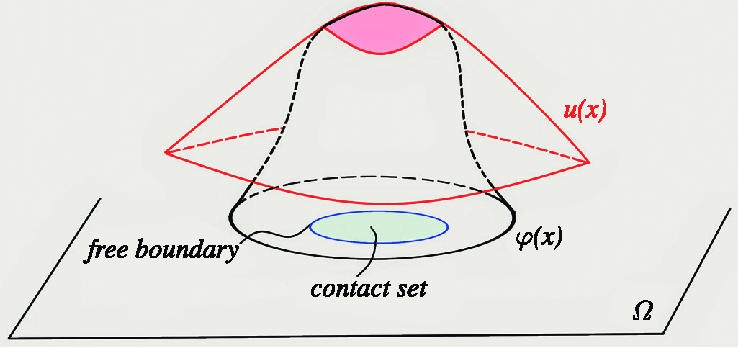
\includegraphics[scale=0.4]{figures/Example-of-an-obstacle-problem.png}
    \caption{Illustrierung eines Hindernis-Problems: Eine ellastische Membran u(x) wird über ein Hindernis \(\varphi(x)\) gespannt; in pink ist die Kontaktmenge dargestellt; diese wird durch eine Karte (in grün-blau) in \(\Omega\) dann dargestellt. \cite{ObstacleProblem}}
    \label{fig:obs}
\end{figure}

Wir werden uns im Folgenden einen Zugang zur Relaxierung mittels Young-Maße schaffen. Doch zunächst sollten wir kurz für das Folgende wichtige Definitionen/Notationen aus der Maßtheorie wiederholen/einführen:\\
\pgfsetfillopacity{0.2}\colorbox{defblue}{\begin{minipage}{16cm}{\textcolor{black}{\pgfsetfillopacity{1}}{\label{def3.1}}}
\textbf{Definition/Notation 3.1:} 
\begin{itemize}
    \item \(\mathcal{C}_0(\mathbb{R}^n) := \overline{\mathcal{C}_c(\mathbb{R}^n)}^{||\cdot||_{\infty}}\).
    \item Sei \(\mathcal{M}^n\) die \(\sigma-\)Algebra aller messbaren Teilmengen \(\Omega\) des \(\mathbb{R}^n\). Der zugehörige Raum ist dann der Banachraum \((\mathcal{M}(\mathbb{R}^n),||\cdot||_{\text{TV}})\) als mit der Totalvariationsnorm normierter Raum aller endlichen signierten Borelmaße auf \(\mathbb{R}^n\). Wir schreiben im Folgenden dann für diesen Raum kurz \(\mathcal{M}(\mathbb{R}^n)\). Hierbei ist die Totalvariationsnorm definiert als
    \begin{equation}
        ||\mu||_{\text{TV}} := \mu^+(\Omega) + \mu^-(\Omega)\, \, \forall \mu \in \mathcal{M}(\mathbb{R}^n),
    \end{equation}
    indem wir \(\mu = \mu^+ - \mu^-\) aus dem Zerlegungssatz von Jordan (siehe Anhang) erhalten.
    \item \(L^{\infty}_{w^*}(\Omega,\,\mathcal{M}(\mathbb{R}^n))\) bezeichnet den Funktionenraum (von Äquivalenzklassen von) schwach*-messbaren, wesentlich beschränkten Funktionen für i.A. \(\Omega \stackrel{messbar}{\subset} \mathbb{R}^n\).
    \item Für allgemeinere Abbildungen \(f:\Omega \to \mathcal{B}\), mit \(\mathcal{B}\) einem Banachraum, definieren wir analog zum Lebesgue-Integral das sogenannte Bochner-Integral auf einem \(\sigma-\)endlichen und vollständigen Maßraum \((\Omega,\Sigma_{\Omega},\mu)\) durch:
    \begin{equation}
        \forall \text{ disjunkten } B_i \in \Sigma_{\Omega}: \int_{\Omega} f \, d\mu := \int_{\Omega} (\sum_{i=1}^n \chi_{B_i}x_i) d\mu := \sum_{i=1}^n \mu(B_i)x_i,
    \end{equation}
\end{itemize}
\end{minipage}}

\begin{figure}[!h]
    \centering
    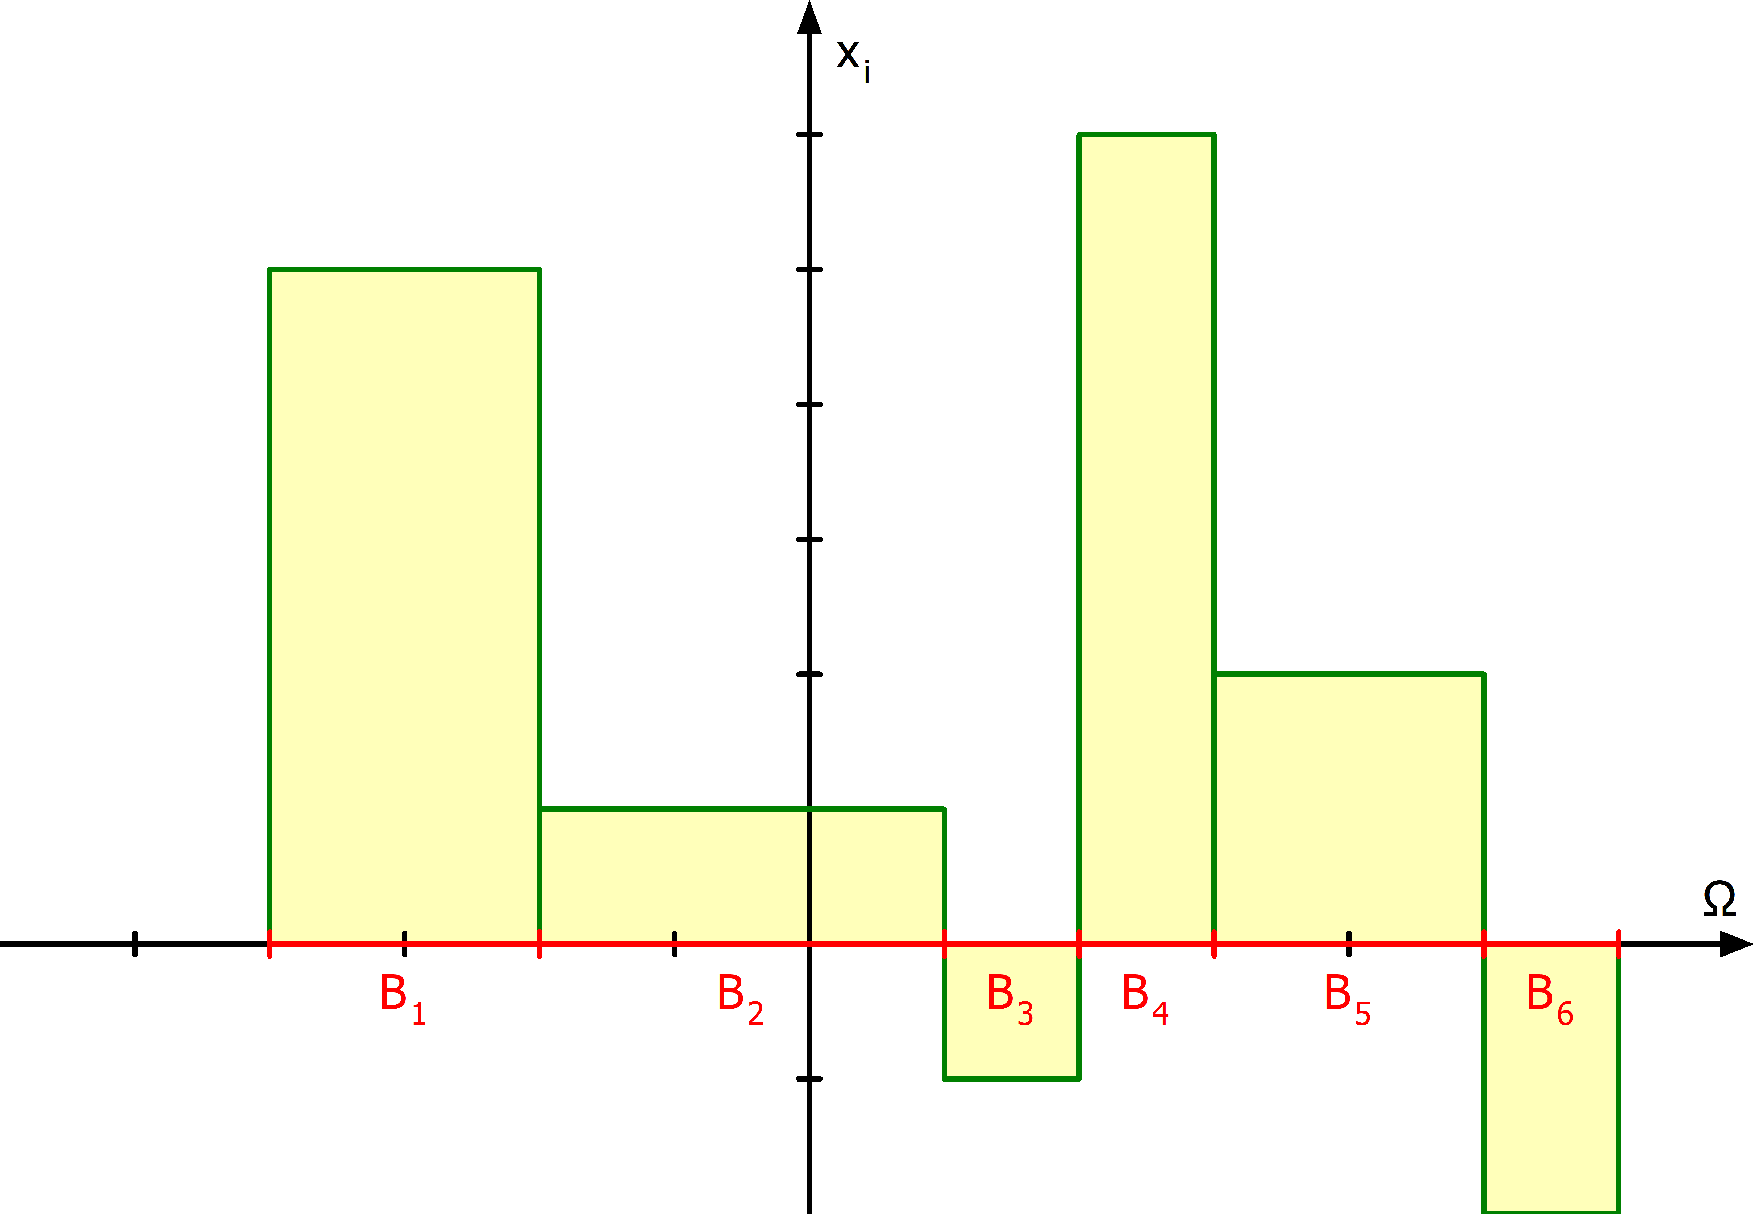
\includegraphics[scale=0.4]{figures/BochnerOhneUrsprungPDF.pdf}
    \caption{Illustration des Bochner-Integrals}
    \label{fig:boch}
\end{figure}

Wir geben nun zwei sehr interessante Resultate für Young-Maße an, von dem eines für die abschließende Betrachtung des Bolza-Problems (1.5) von großer Bedeutung sein wird. Jedoch werden wir aus Zeitgründen diese Resultate nicht beweisen, verweisen für die (nicht uninteressanten) Beweise auf \cite{CalcVarBSchmidt}[Seite 106-109].\\
\pgfsetfillopacity{0.2}\colorbox{theored}{\begin{minipage}{16cm}{\textcolor{black}{\pgfsetfillopacity{1}}{\label{theo3.2}}}
\textbf{Satz 3.2 (Hauptsatz für Young-Maße):} Betrachte \(\Omega \stackrel{messbar}{\subset} \mathbb{R}^n\) und eine messbare Funktionenfolge \(w_k:\Omega \to \mathbb{R}^n\). Dann \(\exists\) Teilfolge \(w_{k_j}\) von \(w_k\), \(\nu \in L^{\infty}_{w^*}(\Omega,\,\mathcal{M}(\mathbb{R}^n))\), sodass gilt:
\begin{enumerate}
    \item \begin{equation}
        \nu_x \geq 0\, \land ||\nu||_{\mathcal{M}(\mathbb{R}^n)} = \int_{\mathbb{R}^n} d\nu_x \le 1\text{ f.f.a. x}
    \end{equation}
    \item \begin{equation}
        \forall f \in \mathcal{C}_0(\mathbb{R}^n):\, f(w_{k_j}) \stackrel{*}{\rightharpoonup} \,<\nu_x,f> \,:= \int_{\mathbb{R}^n} f(y)\,d\nu_x(y)\text{ in }L^{\infty}(\Omega,\,\mathbb{R}^d).
    \end{equation}
\end{enumerate}
\end{minipage}}\\

Das hier erzeugte Maß \(\nu\) erweckt den Eindruck durch die Charakterisierung dieses Hauptsatzes, dass es ein Wahrscheinlichkeitsmaß beschreibt. Und tatsächlich kann man genau das auch zeigen. Benannt wird dieses Maß nach Laurence Chisholm Young, der dieses gefunden hatte:\\
\pgfsetfillopacity{0.2}\colorbox{defblue}{\begin{minipage}{16cm}{\textcolor{black}{\pgfsetfillopacity{1}}{\label{def3.3}}}
\textbf{Definition 3.3 (Young-Maß):} Betrachte eine Familie von Maßen \(\nu := (\nu_x)_{x \in \Omega}\) und eine messbare Funktionenfolge \(w_k:\Omega \to \mathbb{R}^n\). Dann nennen wir die Abbildung
    \begin{equation}
        \nu: \Omega \to \mathcal{M}(\mathbb{R}^n)
    \end{equation}
    das von \(w_{k_j}\) (als Teilfolge von den \(w_k\)) erzeugte Young-Maß.
\end{minipage}}\\

Das Young-Maß ist ziemlich gut reguliert. So trägt es z.B. die starke Regularitäts-Eigenschaft, dass Maß-Konvergenz auf einer kompakten Teilmenge des \(\mathbb{R}^n\) impliziert, dass diese kompakte Menge schon den gesamten Träger des Maßes beinhaltet:\\
\pgfsetfillopacity{0.2}\colorbox{theored}{\begin{minipage}{16cm}{\textcolor{black}{\pgfsetfillopacity{1}}{\label{theo3.4}}}
\textbf{Satz 3.4 (Eigenschaft von Young-Maßen):} Betrachte die gleichen Voraussetzungen wie in [\ref{theo3.2}][Satz 3.2]. Sei zudem \(K \subset \mathbb{R}^n\) kompakt. Dann gilt:
\begin{equation}
    \text{dist}(w_{k_j},K) \stackrel{\nu}{\to} 0 \, \Rightarrow \, \text{supp }\nu_x \subset K\text{ f.f.a. x}.
\end{equation}
\end{minipage}}\\

Wir befinden uns nun in der Situation, in der wir eine maßtheoretische Lösung für die Relaxierung des Bolza-Problems (1.5) beschreiben können. Hierzu betrachten wir der Einfachkeit wegen (1.5) mit a=0, b=1.\\
Betrachte also eine Minimierungsfolge \(u_k\), i.e. \(w_k := u'_k\). Die Voraussetzungen von [\ref{theo3.2}][Satz 3.2] sind erfüllt, also existiert zunächst einmal eine Teilfolge \(w_{k_j}\), die ein Young-Maß \(\nu\) erzeugt. Die Folge \(w_k\) ist beschränkt in \(L^4(]0,1[)\) (Definition Minimierungsfolge), also gilt \(||\nu_x||_{\mathcal{M}(\mathbb{R}^n)} = 1\) (für einen Beweis siehe: \cite{CalcVarBSchmidt}[Seite 106, Bemerkung 3]). Wir wählen für ein \(\epsilon > 0\) nun ein \(\delta > 0\), sodass
\begin{equation}
    (x^2 - 1)^2 < \delta \, \Rightarrow \, \min \{|x-1|,\,|x+1|\} < \epsilon
\end{equation}
gilt. Es folgt:
\begin{equation}
    |\{\text{dist}(w_{k_j},\{-1,1\})\geq \epsilon\}| \le |\{(w^2_{k_j} - 1)^2 \geq \delta\}| \le \frac{1}{\delta} \int_{0}^1 (w^2_{k_j} - 1)^2 \, dx \le \frac{1}{\delta}\mathcal{F}(u_{k_j}) \stackrel{j \to \infty}{\to} 0
\end{equation}
Mit [\ref{theo3.4}][Satz 3.4] folgt supp \(\nu_x \subset \{-1,1\}\) f.f.a. x. Es gilt also:
\begin{equation}
    \exists \lambda(x) \in [0,1]:\,\nu_x = \lambda(x)\delta_{-1} + (1-\lambda(x))\delta_1,
\end{equation}
wobei \(\delta_{(\cdot)}\) das Dirac-Maß bezeichnet. Zudem ist:
\begin{enumerate}
    \item \(u'_{k_j} = w_{k_j} \rightharpoonup w\text{ in }L^4(]0,1[)\)
    \item \(w(x) := \,<\nu_x,id>\, = 1-2\lambda(x)\)
    \item \(\forall \varphi \in \mathcal{C}^{\infty}_c(]0,1[):\, \int_{[0,1]} w\varphi\,dx = \lim_{j \to \infty} \int_{[0,1]} w_{k_j} \varphi\,dx \stackrel{P.I.}{=} 0\)
\end{enumerate}
Für einen Beweis von (1) verweisen wir auf \cite{CalcVarBSchmidt}[Seite 106, Bemerkung 4] (modifizierte Variante von Banach-Alaoglu). Also muss \(w \equiv 0\) gelten (Fundamentallemma) f.ü. und damit ist \(\lambda(x) = \frac{1}{2}\) f.ü. Damit haben wir gezeigt, dass \(w_{k_j}\) das Young-Maß
\begin{equation}
    \nu_x = \frac{1}{2}(\delta_{-1} + \delta_1)\,\,\text{ f.f.a. x}
\end{equation}
erzeugt.\\

Die abschließende Frage ist nun natürlich: Wie hängen das Young-Maß und die Relaxierung von Integralfunktionalen zusammen? Die Antwort ist die Folgende:\\
\pgfsetfillopacity{0.2}\colorbox{theored}{\begin{minipage}{16cm}{\textcolor{black}{\pgfsetfillopacity{1}}{\label{theo3.5}}}
\textbf{Satz 3.5 (Young-Maße und Integralfunktionale):} Sei \(w_k: \Omega \to \mathbb{R}^n\) eine messbare Funktionenfolge, dessen Teilfolge \(w_{k_j}\) das Young-Maß \(\nu\) generiert, \(f \in \mathcal{C}^0(\Omega \times \mathbb{R}^n)\) eine nach unten beschränkte Funktion. Dann gilt:
\begin{enumerate}
    \item \begin{equation}
        \liminf_{k \to \infty} \int_{\Omega} f(x,w_k(x))\,dx \geq \int_{\Omega} \int_{\mathbb{R}^n} f(x,y)\,d\nu_x(y)\,dx
    \end{equation}
    \item Ist zudem \(f(\cdot,w_k(\cdot))\) schwach relativ folgenkompakt in \(L^1(\Omega)\), gilt:
    \begin{equation}
        f(\cdot,w_k) \rightharpoonup \, <\nu_x,f>.
    \end{equation}
\end{enumerate}
\end{minipage}}
    \end{content}
    
    \pagenumbering{Roman}
    \setcounter{page}{\numexpr\value{savepage}}

    % List of figures (if you have figures)
    %\listoffigures
    
    % References
    \references{}
    
    % Appendix
\begin{appendix}
Die folgenden Resultate sind dem Buch von Prof. Alt entnommen \cite{FunkAnaAlt}. Wir beginnen hierbei mit den 2 vermutlich wichtigsten Resultaten - neben dem Darstellungssatz von Riesz - aus der Funktionalanalysis: Der Satz von Hahn-Banach und Banach-Alaoglu:\\ 
\pgfsetfillopacity{0.2}\colorbox{theored}{\begin{minipage}{16cm}{\textcolor{black}{\pgfsetfillopacity{1}}}
\textbf{Satz A.1 (Hahn-Banach):} Sei \(X\) ein \(\mathbb{R}-\)Vektorraum und es gelte:
\begin{enumerate}
    \item \begin{equation}
        p:X \to \mathbb{R} \text{ ist sublinear}.
    \end{equation}
    \item \begin{equation}
        \text{Für einen Vektorunterraum } Y \subset X:\,f:Y \to \mathbb{R} \text{ ist linear}.
    \end{equation}
    \item \begin{equation}
        \forall x \in Y:\,f(x) \le p(x).
    \end{equation}
\end{enumerate}
Dann existiert eine lineare Abbildung \(F:X \to \mathbb{R}\) mit
\begin{equation}
    F(x)=f(x)\,\forall x \in Y\,\,\land\,\, F(x) \le p(x)\,\forall x \in X
\end{equation}
\end{minipage}}
     
\textbf{Bemerkung:} Der Satz benötigt für die gesuchte Fortsetzung das Lemma von Zorn, um zu gewährleisten, dass für eine potentiell \(\infty-\)dimensionale partiell-geordnete Menge ein maximales Element mithilfe des Auswahlaxioms existiert.\\

Aus diesem Satz kann man den wichtigen Trennungssatz dann folgern:\\
\pgfsetfillopacity{0.2}\colorbox{theored}{\begin{minipage}{16cm}{\textcolor{black}{\pgfsetfillopacity{1}}}
\textbf{Korollar A.2 (Trennungssatz):} Sei \((X,||\cdot||)\), kurz \(X\), ein normierter Raum, \(\emptyset \neq M \subset X\) abgeschlossen und \textbf{konvex}, \(x_0 \in M^c\). Dann existiert ein \(x^* \in X^*\) (topologischer Dualraum von \(X\)) und ein \(\alpha \in \mathbb{R}\), sodass gilt:
\begin{equation}
    \Re (<x,x^*>) \le \alpha \,\forall x \in M \,\,\land\,\, \Re (<x_0,x^*>) > \alpha.
\end{equation}
\end{minipage}}

\pgfsetfillopacity{0.2}\colorbox{theored}{\begin{minipage}{16cm}{\textcolor{black}{\pgfsetfillopacity{1}}}
\textbf{Satz A.3 (Banach-Alaoglu):} Dieser Satz besitzt sowohl eine Variante für die schwache als auch die schwach*-Topologie:
\begin{itemize}
    \item Jeder abgeschlossene Ball in einem \textbf{reflexiven} Banachraum ist schwach kompakt.
    \item Jeder abgeschlossene Ball in dem Dual eines normierten Raumes ist schwach* kompakt.
\end{itemize}
\end{minipage}}

\textbf{Bemerkung:} Dieser Satz besitzt natürlich auch eine Folgenversion (dessen schwache Version wir auf Seite 11 auch benutzt haben). Aber Vorsicht: Die schwach* Version benötigt einen \textbf{seperablen} normierten Raum! Diese Zusatzannahme mag zunächst merkwürdig sein; der Grund hierfür ist aber der berüchtigte Problemverursacher \(l^{\infty}\).\\

Für die Variationsrechnung ist bekanntlich die Norm-Topologie zu stark (kompakte Mengen benötigen hier Totalbeschränktheit (Verallgemeinerung des Satzes von Heine-Borel)) und wir suchen für die direkte Methode nach Unterhalbstetigkeit bezüglich der schwachen Topologie. Wir benötigen deshalb in der gesamten Existenztheorie die Annahme der Konvexität. Der Grund liegt im Mazur-Lemma zugrunde, das mithilfe der Resultate A.1, A.2 und A.3 bewiesen werden kann:\\
\pgfsetfillopacity{0.2}\colorbox{theored}{\begin{minipage}{16cm}{\textcolor{black}{\pgfsetfillopacity{1}}}
\textbf{Satz A.4 (Mazur):} Jede \textbf{konvexe} abgeschlossene Menge in einem normierten Raum ist auch schwach abgeschlossen.
\end{minipage}}
\\

Maßtheoretisch sollten wir 2 Aspekte von Seite 8 und einen von Seite 9 noch genauer erklären: Was ist eigentlich ein Caratheodory-Integrand und was ist mit dem Satz von Scorza-Dragoni, sowie dem Zerlegungssatz von Jordan gemeint? Quellen hierfür sind etwas verstreut; gesammelt können die Resultate in \cite{CalcVar} gefunden werden. Der Zerlegungssatz von Jordan ist sehr schön in \cite{ElstrodtMeas}[Seite 271-274] zu finden.\\
\pgfsetfillopacity{0.2}\colorbox{defblue}{\begin{minipage}{16cm}{\textcolor{black}{\pgfsetfillopacity{1}}}
\textbf{Definition A.5 (Caratheodory Funktion):} Wir nennen eine Funktion \\ \(F:\Omega \times \mathbb{R}^N \times \mathbb{R}^{N \times n} \to \mathcal{X}\) mit \(\Omega \stackrel{messbar}{\subset} \mathbb{R}^n\) und metrisierbaren Raum \(\mathcal{X}\) Caratheodory Funktion, falls gilt:
\begin{enumerate}
\item \begin{equation}
    F(x,\cdot, \cdot):\mathbb{R}^N \times \mathbb{R}^{N \times n} \to \mathcal{X} \text{ ist stetig f.ü. und}
\end{equation}
\item \begin{equation}
    F(\cdot,y,z):\Omega \to \mathcal{X} \text{ ist messbar }\forall (y,z) \in \mathbb{R}^N \times \mathbb{R}^{N \times n}.
\end{equation}
\end{enumerate}
\end{minipage}}

Um den Satz von Scorza-Dragoni zu beweisen, benötigt man 2 Sätze, namentlich den Satz von Luzin und den Satz von Egorov:\\
\pgfsetfillopacity{0.2}\colorbox{theored}{\begin{minipage}{16cm}{\textcolor{black}{\pgfsetfillopacity{1}}}
\textbf{Satz A.6 (Luzin):} Betrachte \(\Omega \stackrel{offen}{\subset} \mathbb{R}^n\) mit \(\mathcal{L}^n(\Omega) < \infty\), einen metrisierbaren Raum \(\mathcal{X}\) und eine messbare Funktion \(f:\Omega \to \mathcal{X}\). Dann gilt:
\begin{equation}
    \forall \epsilon > 0\,\exists A \stackrel{kompakt}{\subset} \Omega \text{ mit } \mathcal{L}^n(A^c) < \epsilon, \text{ sodass } f_{\einschraenkung A} \text{ stetig ist}.
\end{equation}
\end{minipage}}

\pgfsetfillopacity{0.2}\colorbox{theored}{\begin{minipage}{16cm}{\textcolor{black}{\pgfsetfillopacity{1}}}
\textbf{Satz A.7 (Egorov):} Betrachte \(\Omega \stackrel{offen}{\subset} \mathbb{R}^n\) mit \(\mathcal{L}^n(\Omega) < \infty\), einen metrisierbaren Raum \(\mathcal{X}\) und messbare Funktionen \(f,f_k: \Omega \to \mathcal{X}\), sodass \(f_k \stackrel{k \to \infty}{\to} f\) f.ü. Dann gilt:
\begin{equation}
    \forall \epsilon > 0 \,\exists B \stackrel{kompakt}{\subset} \Omega \text{ mit } \mathcal{L}^n(B^c) < \epsilon, \text{ sodass } f_k \stackrel{k \to \infty}{\to} f \text{ gleichmäßig auf } B.
\end{equation}
\end{minipage}}

Der Satz von Scorza-Dragoni kann dann hauptsächlich durch iteratives Anwenden von A.6 bewiesen werden und lautet:\\
\pgfsetfillopacity{0.2}\colorbox{theored}{\begin{minipage}{16cm}{\textcolor{black}{\pgfsetfillopacity{1}}}
\textbf{Satz A.8 (Scorza-Dragoni):} Betrachte \(\Omega \stackrel{offen}{\subset} \mathbb{R}^n\) mit \(\mathcal{L}^n(\Omega) < \infty\), einen metrisierbaren Raum \(\mathcal{X}\) und eine Caratheodory Funktion \(F:\Omega \times \mathbb{R}^N \to \mathcal{X}\). Dann gilt:
\begin{equation}
    \forall \epsilon > 0\,\exists A \stackrel{kompakt}{\subset} \Omega \text{ mit } \mathcal{L}^n(A^c) < \epsilon, \text{ sodass } F_{\einschraenkung A \times \mathbb{R}^N} \text{ stetig ist}.
\end{equation}
\end{minipage}}

Abschließend noch der Zerlegungssatz von Jordan, der den Zerlegungssatz von Hahn verwendet:\\
\pgfsetfillopacity{0.2}\colorbox{theored}{\begin{minipage}{16cm}{\textcolor{black}{\pgfsetfillopacity{1}}}
\textbf{Satz A.9 (Hahn):} Sei \((X,\Sigma,\mu)\) ein Maßraum mit einem signierten Maß \(\mu: \Sigma \to \overline{\mathbb{R}}\). Dann existiert eine disjunkte Zerlegung \(X=P \cup N\) mit \(P,N \in \Sigma\) von \(X\) in eine positive Menge \(P\) und eine negative Menge \(N\).
\end{minipage}}

\pgfsetfillopacity{0.2}\colorbox{theored}{\begin{minipage}{16cm}{\textcolor{black}{\pgfsetfillopacity{1}}}
\textbf{Satz A.10 (Jordan):} Jedes signierte Maß \(\mu\) eines Maßraums \((X,\Sigma,\mu)\) besitzt die Jordan-Zerlegung
\begin{equation}
    \mu = \mu^+ - \mu^-,
\end{equation}
wobei \(\mu^+ \perp \mu^-\) gilt.
\end{minipage}}
\end{appendix}

    % Declaration of authorship
    % \authorshipstatement[pagenumbering=false]
    \authorshipstatement[pagenumbering=true]
    % \authorshipstatement[pagenumbering=only]
    
    % Consent form for use of plagiarism detection software
    % Not yet required
    % \consentform[pagenumbering=false]
    % \consentform[pagenumbering=true]
    % \consentform[pagenumbering=only]
    
    % Bonus: Wordcount
    % cd %FOLDER WHERE THE .tex FILES ARE IN %
    % clear
    % texcount -total -q -col -sum *.tex
    
\end{document}